% results_ts.tex — Elicit vs. teach inside one model family (TinyStories-1B),
% organised by METRIC. Each metric has the same three blocks: "Elicit vs. teach,
% in one sentence" (what the metric asks and which way each regime falls), "How
% it is measured" (the procedure, self-contained), "The numbers" (the headline
% values, a pointer to the table or figure, and a one-line reading). Figures are the PNGs generated by make_assets.py in this
% figures/ subfolder next to this file (copied from the make_assets.py output). Every number has a dated entry in
% ../notes/decisions.md.
\documentclass[11pt]{article}
\usepackage{amsmath,amssymb}
\usepackage{graphicx}
\usepackage{booktabs}
\usepackage{adjustbox}
\usepackage[margin=1in]{geometry}
\usepackage{enumitem}
\usepackage{hyperref}
\newcommand{\what}[1]{\par\noindent\textbf{Elicit vs.\ teach, in one sentence.} #1}
\newcommand{\how}[1]{\par\noindent\textbf{How it is measured.} #1}
\newcommand{\numbers}[1]{\par\noindent\textbf{The numbers.} #1\par\medskip}
\newcommand{\metricsec}[2]{\item \textbf{#1} --- \emph{#2}}

\title{Elicit vs.\ Teach, Mechanistically:\\ Ten Metrics on the TinyStories-1B Twins}
\author{MARS V --- Mechanistic Understanding of Elicitation vs.\ Teaching}
\date{Working results document, September 2026}

\begin{document}
\maketitle

\section*{Setup}

\noindent\textbf{The experiment.} Two identical copies (``twins'') of a 1B-parameter language model
pretrained only on children's stories --- no arithmetic anywhere in the corpus --- are fine-tuned
on the same target task: natural-language addition and subtraction of 1--4-digit numbers,
\texttt{What is the difference between 8 and 5784?}$\;\to\;$\texttt{-5776}. The training protocol
is identical for both. The \emph{only} difference is the checkpoint the fine-tune starts from:

\begin{itemize}[nosep]
  \item \textbf{Teach twin}: the blank base model. The capability is absent.
  \item \textbf{Elicit twin} (``TS1B-latent''): the blank base plus two installations, neither of
    which shows the target task: (i) arithmetic in symbols only (\texttt{23 + 45 = 68}, 1M
    examples, full fine-tuning) and (ii) a word$\leftrightarrow$symbol binding dose that only
    \emph{rewrites} questions (\texttt{What is the sum of 621 and 5068?} $\leftrightarrow$
    \texttt{621 + 5068}) and never shows an answer. This twin can compute in symbols and knows
    what the words mean, but on the target task it scores $0.000$: asked a question, it rewrites
    it instead of answering. The capability is latent.
\end{itemize}

\noindent Every construction step has a control (Table~\ref{tab:premise}); the two twins are
behaviourally identical on the target task before fine-tuning.

\begin{table}[h]\centering\small
\begin{adjustbox}{max width=\textwidth}
\begin{tabular}{lcc}
\toprule
Construction step / check & value & control \\
\midrule
symbol install: exact match on \texttt{23 + 45 = } & 0.67--0.73 & blank twin: 0.00 \\
corpus census: ``sum'' in 439M words of stories & 21$\times$ & ``equals'' 17, ``minus'' 57 \\
binding dose: question $\to$ symbols rewrite exact & 0.484 & blank + same dose: 0.000 \\
sum-only dose on \emph{difference} questions & writes ``+'' & binding is per word \\
self-chain: rewrite the question, then feed the model its own rewrite & 0.328 ($=0.484\times0.668$) & blank + same doses: 0.000 \\
\textbf{exact match on the target task, before fine-tuning} & \textbf{0.000} & $=$ blank twin \\
\bottomrule
\end{tabular}
\end{adjustbox}
\caption{The elicit twin before fine-tuning: can compute in symbols, understands the words, still
answers nothing --- and the two parts compose (self-chain $=$ rewrite accuracy $\times$ symbol
accuracy, a product that held on four variants). Everything below is
about what differs inside the two twins and what that difference does.}
\label{tab:premise}
\end{table}

\noindent\textbf{The pair every metric is reported on.} The teach parent used throughout is the
\emph{format-installed} twin: the blank base first fine-tuned on a random-label dose in the
target's own format, so that it already emits a number after every question (format validity
$1.000$) without ever having seen a correct one (exact match $0.000$). This is the paper's
``pre-teach format'' control and makes the two parents design-matched: both are the blank base
plus one full-fine-tuning dose, both already output numbers, only one has the algorithm. Both
parents are then fully fine-tuned with the identical recipe on the identical 4M-example file to
convergence: \textbf{elicit FT} reaches exact match $0.986$ in 21,500 steps; \textbf{teach FT}
reaches $0.424$ in 58,500 steps (Table~\ref{tab:endpoints}). Teaching this base needs full
fine-tuning: under the paper's adapter protocol (LoRA) the taught twin stops by its own
convergence rule at $0.09$--$0.14$, where the paper's Figure~2 puts it. Other endpoints appear
only where they add something: the LoRA runs carry the learning-curve sweeps and the training
snapshots (M1, M4, M6), and the teach twin fine-tuned from the \emph{blank} base ($0.819$) is
the control that separates the algorithm from the format (M7) and the robustness check in
Section~E.

\begin{table}[h]\centering\small
\begin{adjustbox}{max width=\textwidth}
\begin{tabular}{llllccc}
\toprule
endpoint & parent & method & data & steps (passes) & stop & exact match \\
\midrule
\textbf{elicit FT} & TS1B-latent & full FT & 4M & 21{,}500 (0.7) & converged & \textbf{0.986} \\
\textbf{teach FT} & format-installed & full FT & 4M & 58{,}500 (1.9) & converged & \textbf{0.424} \\
\midrule
elicit LoRA (sweep, snapshots) & TS1B-latent & LoRA $r{=}512$ & 1M & 11{,}500 (1.5) & converged & 0.981 \\
teach LoRA (sweep) & format-installed & LoRA $r{=}512$ & 1M & -- & converged & 0.079 \\
teach LoRA (snapshots) & blank & LoRA $r{=}512$ & 1M & 25{,}000 (3.2) & converged & 0.093 \\
teach FT from the blank base (control) & blank & full FT & 4M & 72{,}000 (2.3) & converged & 0.819 \\
\bottomrule
\end{tabular}
\end{adjustbox}
\caption{The main pair (top) and the endpoints used where noted (bottom). LoRA learning rate
$3.53{\times}10^{-4}$, full FT $2{\times}10^{-5}$; batch 128; seed 316; training stops when
validation loss stops improving (eps/k rule). Exact match $=$ 0-shot accuracy on 1,024 held-out
problems. The 4M file is the 1M file plus 3M new unique problems, disjoint from every evaluation
set.}
\label{tab:endpoints}
\end{table}

\noindent\textbf{Two terms used throughout.} \emph{Answer position}: the last prompt token, where
the model predicts the first token of the answer; every activation measurement is taken there
unless stated. \emph{Residual stream}: the model's running internal state at a token position, a
2048-dimensional vector that every layer reads and adds to. Everything else is defined where it
is used.

\noindent\textbf{How to read this document.} Ten metrics, each with the same three blocks:
\textbf{Elicit vs.\ teach, in one sentence} (what the metric asks and which way each regime
should fall), \textbf{How it is measured} (the procedure, complete enough to reproduce),
\textbf{The numbers} (elicit FT vs teach FT; every value is in the table or figure it points
to; other endpoints only where they add a control or an intuition). The metrics are grouped
by what they look at: the \emph{cost} of learning (M1), the \emph{machinery} that results
(M2--M3), the \emph{dynamics} of building it (M4--M7), and the \emph{latent state} before any
target training (M8--M10). Table~\ref{tab:ftpair} at the end puts every metric for the pair on one
page, with the robustness endpoints beside it.

% =====================================================================
\section*{A. Cost of learning}
\begin{enumerate}[label=\textbf{M\arabic*}, leftmargin=*, itemsep=1.2em]

\metricsec{Learning cost}{cheaper with every example vs.\ the hump}
\what{Does each new example cost less than the last, because it only connects a capability that
exists (elicit), or does the cost first rise, because structure is being built (teach)?}
\how{Prequential excess description length (EDL), the paper's learning-cost measure. Train on a
stream of $n$ examples; before each example is trained on, record the extra nats the model needs
to predict its answer tokens beyond a converged reference; sum over the stream and divide by the
number of answer tokens (EDL per token). Repeat on a sweep $n=100\ldots4{\times}10^6$ with the
identical LoRA protocol (19 rungs per arm, all converged), plus 0-shot exact match on 1,024
held-out problems at each rung. A falling curve means each example costs less than the last; a
down--up--down curve (``the hump'') means mid-run examples are the most informative because
structure is being built. Two arms: the elicit twin and the format-installed teach twin; the blank teach twin's sweep is
shown alongside to make the format's share of the cost visible. The full-FT endpoints have no
sweep; their cost is reported as steps to convergence and held-out test loss.}
\numbers{Figure~\ref{fig:flip}, Table~\ref{tab:sweep}. EDL/token falls monotonically for the
elicit twin ($4.53\to0.09$) and goes down--up--down for the teach twin (minimum $0.64$ at 10K,
peak $1.33$ at 100K, $0.88$ at 1M). Exact match at 1M: $0.98$ vs $0.08$; under full FT $0.986$
vs $0.424$, in $0.7$ vs $1.9$ passes. The blank teach twin has the same hump, higher ($0.78$ /
$2.02$ / $1.40$): the format is a fixed cost on top, not the hump. \emph{Reading:} eliciting
connects a capability that exists; teaching builds one, and the hump is the algorithm being
built.}
\begin{figure}[h]\centering
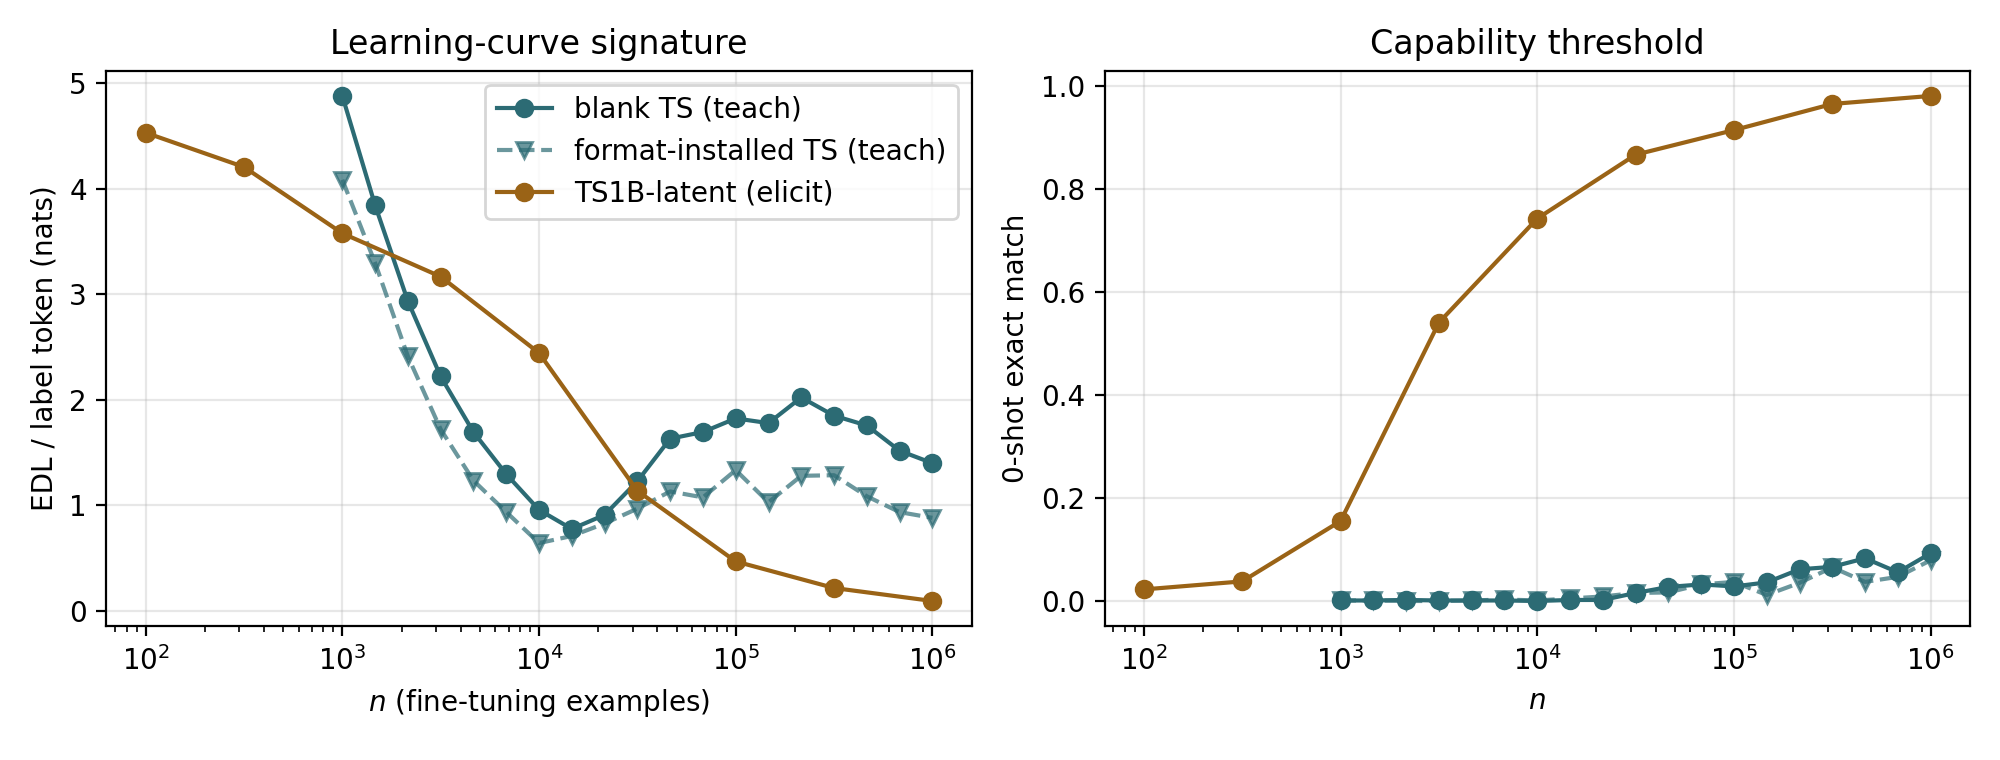
\includegraphics[width=\textwidth]{figures/fig_signature_flip.png}
\caption{EDL/token (left) and 0-shot exact match (right) vs $n$; teal = teach twin from the blank base, dashed teal = teach twin from the format-installed base, gold = elicit twin.}
\label{fig:flip}
\end{figure}
\begin{table}[h]\centering\small
\begin{adjustbox}{max width=\textwidth}
\begin{tabular}{rcccccc}
\toprule
$n$ & \multicolumn{2}{c}{elicit (TS1B-latent)} & \multicolumn{2}{c}{teach (blank)} & \multicolumn{2}{c}{teach (format-installed)} \\
 & EDL/tok & EM & EDL/tok & EM & EDL/tok & EM \\
\midrule
100 & 4.533 & 0.023 & 6.511 & 0.007 & -- & -- \\
316 & 4.208 & 0.038 & 6.387 & 0.033 & -- & -- \\
1{,}000 & 3.579 & 0.155 & 4.882 & 0.001 & 4.087 & 0.001 \\
3{,}162 & 3.168 & \textbf{0.541} & 2.221 & 0.001 & 1.720 & 0.000 \\
10{,}000 & 2.444 & 0.743 & 0.956 & 0.000 & \emph{0.641} (min) & 0.001 \\
14{,}678 & -- & -- & \emph{0.775} (min) & 0.002 & 0.708 & 0.005 \\
31{,}623 & 1.137 & 0.867 & 1.228 & 0.016 & 0.968 & 0.016 \\
100{,}000 & 0.467 & 0.915 & 1.824 & 0.028 & \emph{1.333} (peak) & 0.037 \\
215{,}443 & -- & -- & \emph{2.022} (peak) & 0.062 & 1.279 & 0.035 \\
316{,}228 & 0.215 & 0.966 & 1.849 & 0.066 & 1.285 & 0.065 \\
1{,}000{,}000 & \textbf{0.092} & \textbf{0.981} & 1.399 & 0.093 & 0.880 & 0.079 \\
4{,}000{,}000 & -- & -- & 0.930 & 0.139 & -- & -- \\
\bottomrule
\end{tabular}
\end{adjustbox}
\caption{Per-rung values, LoRA protocol (EDL in nats per answer token; EM $=$ exact match; 19
rungs per teach arm, all converged; rungs shared with the elicit sweep shown plus each arm's
minimum and peak).}
\label{tab:sweep}
\end{table}

% =====================================================================
\end{enumerate}
\section*{B. The machinery that results}
\begin{enumerate}[label=\textbf{M\arabic*}, leftmargin=*, itemsep=1.2em, resume]

\metricsec{Circuit overlap}{the same circuit vs.\ a new circuit}
\what{Does the fine-tuned model solve the task with the circuit its parent already had (elicit)
or with a circuit that did not exist before (teach)?}
\how{\emph{Building a circuit.} The model is split into 528 nodes: 512 attention heads (32 per
layer $\times$ 16 layers; heads move information between token positions) and 16 MLP blocks (one
per layer; they transform it in place). For each node, attribution patching scores how much the
answer's logit would change if that node's activation at the answer position were replaced by its
value on a different problem: gradient of the answer logit-difference with respect to the node's
activation, times the activation difference between the clean and the corrupted problem, averaged
over 128--256 problem pairs. The 32 highest-scoring nodes are the circuit. A model that cannot do
the task gives a noise map, which the tool flags (its answer logit-difference is $\approx0$).
\emph{Comparing circuits.} Jaccard@32 $=$ shared nodes $\div$ union of the two 32-node sets. Two
random circuits overlap at $0.031$. The \emph{ceiling} is the overlap of two circuits of the
\emph{same} model computed from two disjoint halves of the data --- how repeatable a circuit is
($0.42$--$0.68$ here); an overlap at the ceiling means ``the same circuit''. Spearman $=$ rank
correlation of the node scores over the union. Also which layers and node types each circuit's top nodes come from.}
\numbers{Table~\ref{tab:overlap}. Elicit: parent $\leftrightarrow$ child $0.391$ (score
correlation $0.44$), at the parent map's own repeatability ceiling of $0.306$; nine of the
child's top sixteen nodes are the parent's, led by the same \texttt{mlp:15,14,13,12} --- the
child runs the parent's symbol circuit re-weighted, and the same circuit whichever way it is
trained (LoRA $\leftrightarrow$ full FT $0.641$, at the ceiling). Teach: parent
$\leftrightarrow$ child undefined --- the parent has no circuit for the task (its map fails the
performing-regime check, answer logit-diff $-1.5$; the $0.231$ it scores against its child is
noise overlap), so the child's circuit ($0.52$ repeatable) is new. The two children against each
other: $0.306$. What the two children share is
the late-layer MLP engine (\texttt{mlp:15,14,13,7}); the taught circuit adds early and middle
MLPs (\texttt{mlp:0,1,3,4,5,6,10,11}) and attention heads in layers 4--7 and 15 of its own, the
elicited one uses \texttt{mlp:8,9} and three layer-7 heads. \emph{Reading:} elicitation
re-weights the circuit the parent already had; teaching builds a related but different one.}
\begin{table}[h]\centering\small
\begin{adjustbox}{max width=\textwidth}
\begin{tabular}{lccc}
\toprule
Comparison & Jaccard@32 & chance & ceiling(s) \\
\midrule
\textbf{elicit parent (symbol circuit) $\leftrightarrow$ elicited child (FT)} & \textbf{0.391} (Spearman 0.44) & 0.031 & 0.306 / 0.561 \\
\textbf{teach parent $\leftrightarrow$ taught child (FT)} & \textbf{undefined}: the parent's map is noise (answer logit-diff $-1.5$; noise overlap 0.231) & 0.031 & -- / 0.524 \\
\midrule
elicit parent (symbol circuit) $\leftrightarrow$ elicited child (LoRA) & 0.455 (Spearman 0.59) & 0.031 & 0.306 / 0.684 \\
elicited child (FT) $\leftrightarrow$ taught child (FT) & 0.306 (Spearman 0.03) & 0.031 & 0.561 / 0.524 \\
elicited child, full FT $\leftrightarrow$ elicited child, LoRA & 0.641 (Spearman 0.54) & 0.031 & 0.561 / 0.684 \\
taught child (FT) $\leftrightarrow$ taught child from the blank base (FT) & 0.362 (Spearman 0.18) & 0.031 & 0.524 / 0.422 \\
\bottomrule
\end{tabular}
\end{adjustbox}
\caption{Circuit overlaps. Top: parent $\leftrightarrow$ child in each regime; ceilings are
given for both maps (parent / child). The elicit parent's symbol-task map is itself only $0.306$
repeatable at 32 nodes ($0.40$ at 128), so $0.391$ is at the parent's own ceiling. The teach
parent's map fails the performing-regime check (the tool flags it: its overlap measures noise).
Bottom: the LoRA elicited child against the same parent, the two children against each other,
the elicited circuit under the two methods, and two taught circuits against each other.}
\label{tab:overlap}
\end{table}

\metricsec{Head roles}{the same reader heads vs.\ rediscovered ones}
\what{Does the fine-tuned model keep the parent's heads that read the two numbers (elicit) or
have to find reader heads of its own (teach)?}
\how{Desiderata Component Masking (Prakash et al.\ 2024). For one piece of information at a
time, take a problem and a counterfactual problem that differs only in that piece, and learn
(by gradient descent on a mask over heads, with a sparsity penalty) the smallest set of
attention heads such that copying those heads' activations from the counterfactual run into the
clean run makes the model answer the counterfactual problem. That set is the heads carrying that
piece (its ``role''). The set is validated by its counterfactual-flip accuracy against the
ceiling obtained by copying every head; a set is ``compact'' only if it reaches that ceiling.
Role sets are compared across models by Jaccard (chance $\approx0.05$); 64--128 counterfactual
pairs, heads only.}
\numbers{Table~\ref{tab:dcm}. Both children have compact operand-reading sets at their
ceilings. The elicited child's are the parent's: $0.69$ / $0.86$ overlap with the engine's sets
(first / second operand) under full FT, $0.88$ / $0.90$ under LoRA, all at ceiling flip
accuracy. The taught child's sets are larger (32 / 41 heads vs 30 / 27) and contain most of the
same heads: $0.88$ / $0.66$ vs the engine. A taught model that did not learn the task (LoRA,
exact match $0.14$) has no compact set at all (flip accuracy $0.01$--$0.03$ against a ceiling of
$0.14$--$0.20$). \emph{Reading:} operand reading is a layer-0 function of the substrate;
elicitation keeps it intact, teaching has to find it again and lands on a larger set --- a graded
difference, not an absence.}
\begin{table}[h]\centering\small
\begin{adjustbox}{max width=\textwidth}
\begin{tabular}{lcccc}
\toprule
Comparison (first operand / second operand) & $|A|$ & $|B|$ & Jaccard & flip acc.\ / ceiling of $A$ \\
\midrule
\textbf{elicited child (FT) $\leftrightarrow$ engine} & 31 / 25 & 30 / 27 & \textbf{0.694 / 0.857} & 0.98 / 0.98 (at ceiling) \\
\textbf{taught child (FT) $\leftrightarrow$ engine} & 32 / 41 & 30 / 27 & \textbf{0.879 / 0.659} & 0.59 / 0.54 (0.59 / 0.55) \\
taught child (FT) $\leftrightarrow$ elicited child (LoRA) & 32 / 41 & 36 / 30 & 0.659 / 0.690 & -- \\
\midrule
engine $\leftrightarrow$ elicited child (LoRA), symbol surface & 30 / 27 & 32 / 30 & 0.879 / 0.900 & at ceiling \\
engine $\leftrightarrow$ elicited child (LoRA), operation role & 25 & 24 & 0.750 & at ceiling \\
elicited child (FT) $\leftrightarrow$ elicited child (LoRA) & 31 / 25 & 36 / 30 & 0.811 / 0.833 & 0.98 / 0.98 \\
taught child that did not learn (LoRA 4M) $\leftrightarrow$ elicited child (LoRA) & 12 / 21 & 36 / 30 & 0.043 / 0.041 & 0.01 / 0.03 (0.20 / 0.14) \\
\bottomrule
\end{tabular}
\end{adjustbox}
\caption{Head roles by Desiderata Component Masking. ``Engine'' $=$ the elicit parent on the
symbol surface, the reference role sets. $|A|$, $|B|$ $=$ size of the two role sets. Bottom: the
references (the LoRA-elicited child keeps the engine's roles almost exactly; a taught model that
never learned the task has no roles to compare).}
\label{tab:dcm}
\end{table}

% =====================================================================
\end{enumerate}
\section*{C. Dynamics: how the machinery comes into being}
\begin{enumerate}[label=\textbf{M\arabic*}, leftmargin=*, itemsep=1.2em, resume]

\metricsec{Circuit formation time}{present at step 1 vs.\ assembled mid-run}
\what{Is the final circuit present from the first step (elicit) or assembled somewhere in the
middle of training (teach)?}
\how{Adapter snapshots were saved along the LoRA runs (128 per run, log-spaced); the full-FT
runs have no snapshots, so this metric is read on the LoRA pair (elicit twin vs blank teach
twin, 1M examples each). For each snapshot, build the circuit exactly as in M2 and take its
Jaccard@32 with the run's final circuit; read against chance ($0.031$) and the split-half
ceiling. The step at which the curve leaves the noise floor is when the circuit starts to exist;
the step at which it reaches the ceiling is when it stops changing.}
\numbers{Figure~\ref{fig:form}. Elicit: $0.49$ overlap with the final circuit at step 1
($16\times$ chance), locked from step 1.5K of 11.5K. Teach: at the noise floor until step 1.3K,
then built over steps 1.3K--5.4K, where its EDL peaks (M1). \emph{Reading:} the elicited circuit
is present before training starts; the taught circuit is assembled mid-run, exactly while the
learning cost is rising.}
\begin{figure}[h]\centering
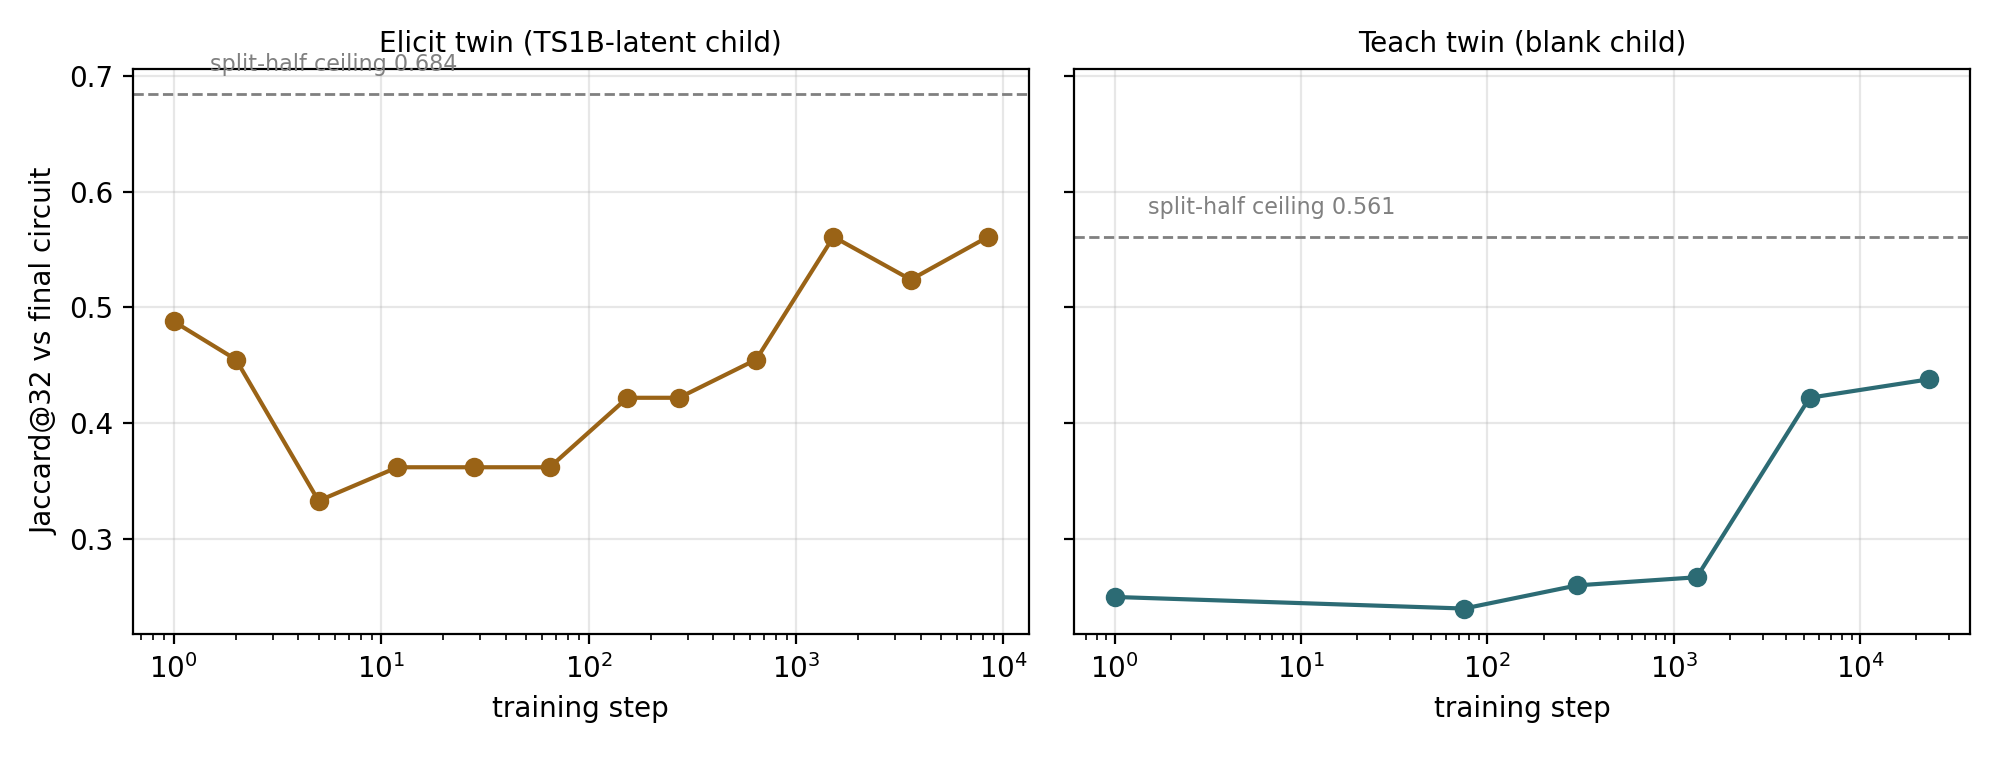
\includegraphics[width=\textwidth]{figures/fig_formation_ts.png}
\caption{Circuit formation, elicit (left) vs teach (right); dashed = split-half ceiling.}
\label{fig:form}
\end{figure}

\metricsec{Gradient pressure}{a dying gradient vs.\ a growing one}
\what{Does the gradient fade as training proceeds because there is nothing left to change
(elicit), or grow because structure is still being built (teach)?}
\how{The global gradient norm before clipping, logged at every update. Reported: its peak and
the step of the peak; its mean over the first 1\%, the middle, and the last 10\% of steps; the
ratio first-1\% $\div$ last-10\% (above 1 $=$ decays, below 1 $=$ grows); and the cumulative
gradient mass $\sum_t\|g_t\|$. For the LoRA runs also how that mass splits across attention
query/key weights (QK), attention value/output weights (VO) and MLP weights; the full-FT trainer
logs the global norm only. Norms are comparable within a method, not across methods (different
parameter sets).}
\numbers{Table~\ref{tab:grad}, Figure~\ref{fig:grad}. Elicit: the gradient peaks at step 1
($34.0$) and decays $3.4\times$ from the first 1\% of steps to the last 10\%. Teach: it starts
lower ($2.7$), peaks at step 50,860 ($70.9$) and ends $1.4\times$ above its start. Cumulative
gradient mass $44$K vs $378$K ($8.6\times$). Under LoRA the same shape with a larger gap ---
elicit decays $3.3\times$, teach grows $40\times$, mass $150\times$ --- and the LoRA logs show where
the teach gradient goes: attention value/output weights (share $0.87$), the operand-fetching
heads of M3 being written. \emph{Reading:} elicitation converges and its gradient dies; teaching
keeps generating pressure while the structure is built.}
\begin{table}[h]\centering\small
\begin{adjustbox}{max width=\textwidth}
\begin{tabular}{lcccc}
\toprule
 & \textbf{elicit FT} & \textbf{teach FT} & elicit LoRA 1M & teach LoRA 1M (blank) \\
\midrule
steps & 21{,}500 & 58{,}500 & 11{,}500 & 25{,}000 \\
peak gradient norm (step) & 34.0 (1) & 70.9 (50{,}860) & 0.441 (96) & 17.4 (23{,}657) \\
mean norm: first 1\% / middle / last 10\% & 4.80 / 1.85 / 1.39 & 2.69 / 4.86 / 3.77 & 0.183 / 0.060 / 0.056 & 0.169 / 5.21 / 6.80 \\
first 1\% $\div$ last 10\% & $\times$3.4 (decays) & $\times$0.7 (grows 1.4$\times$) & $\times$3.3 (decays) & $\times$0.02 (grows $\sim$40$\times$) \\
cumulative gradient mass $\sum_t\|g_t\|$ & 44{,}021 & 378{,}170 & 783 & 116{,}877 \\
gradient mass per step & 2.05 & 6.46 & 0.068 & 4.68 \\
mass share QK / VO / MLP & -- & -- & .18 / .55 / .27 & .12 / .87 / .01 \\
\bottomrule
\end{tabular}
\end{adjustbox}
\caption{Raw gradient strength (pre-clip global norm at every update). LoRA and full-FT norms are
on different parameter sets and are compared within a method only; the LoRA pair is shown for
the per-class split, which the full-FT trainer does not log.}
\label{tab:grad}
\end{table}
\begin{figure}[h]\centering
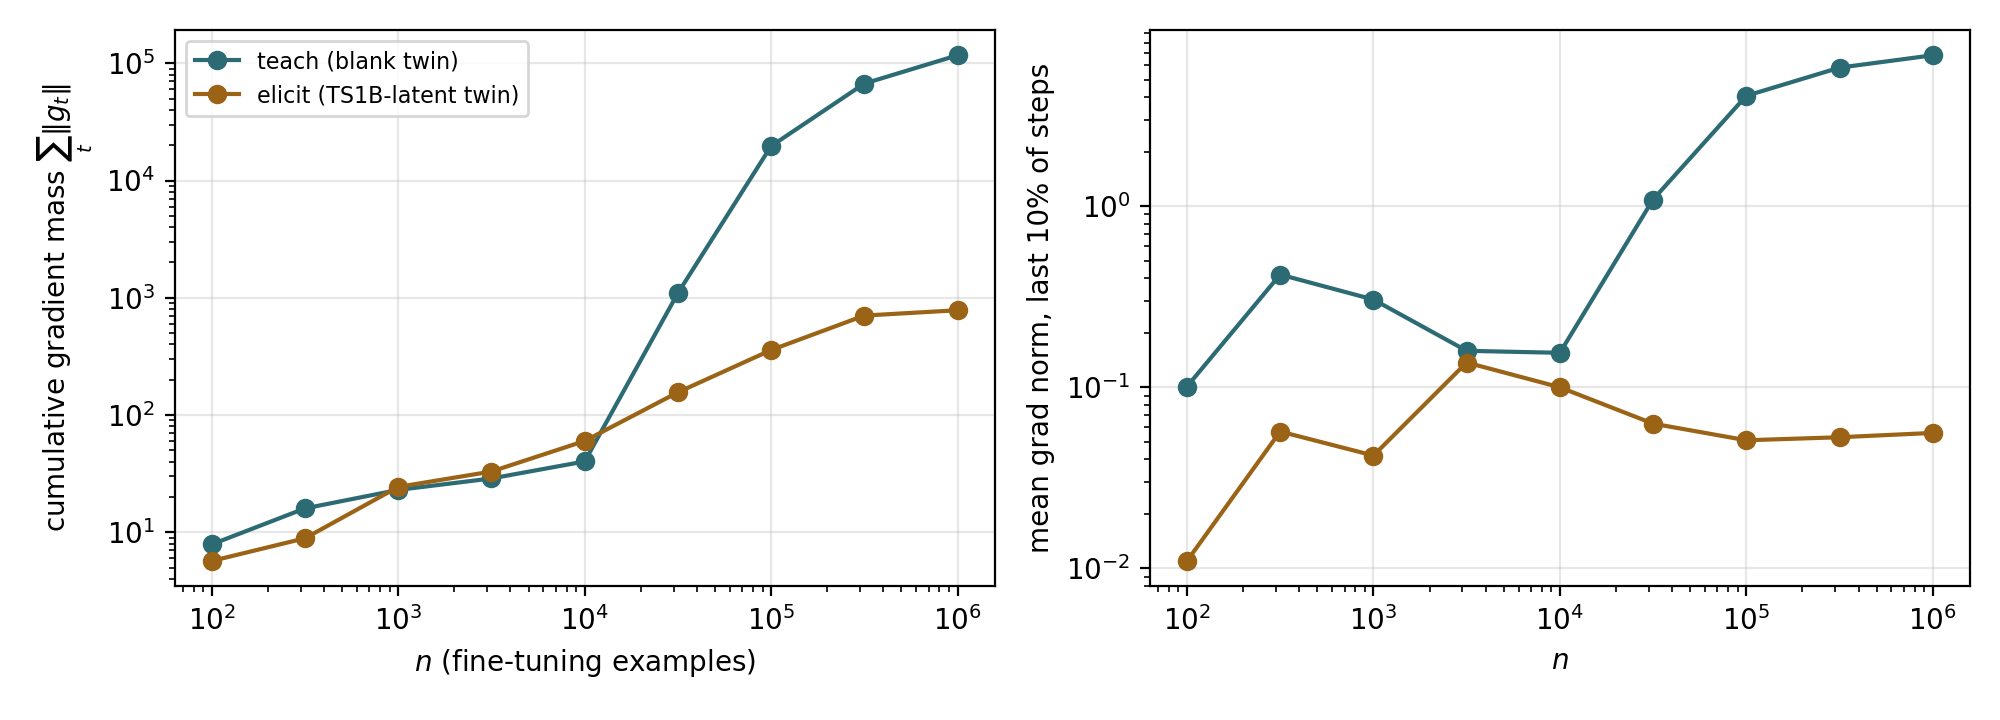
\includegraphics[width=\textwidth]{figures/fig_grad_strength.png}
\caption{Cumulative gradient mass (left) and late-run gradient norm (right) vs $n$; teal = teach, gold = elicit.}
\label{fig:grad}
\end{figure}

\metricsec{Weight write}{a small update vs.\ a large one}
\what{Is the change to the weights small and efficient (elicit) or large and expensive per unit
of capability gained (teach)?}
\how{Relative weight change $\|\Delta W\|/\|W\|$ between child and parent --- exact from the LoRA
factors ($\Delta W = BA$), or from the checkpoint difference for full fine-tuning --- over all
attention and MLP matrices. Along the LoRA runs, from the adapter snapshots: total travel
$\|\Delta W_t\|_F$ vs step, its peak and final speed per step, and capability per unit travel
$=$ final exact match $\div$ total travel.}
\numbers{Table~\ref{tab:weights}. Relative weight write $0.050$ (elicit) vs $0.086$ (teach),
$1.7\times$. The travel instrument exists only
for the LoRA runs (elicit vs blank teach, 1M): write $0.095$ vs $0.212$, travel $120$ vs $457$,
capability per unit travel $8.1\times10^{-3}$ vs $2.0\times10^{-4}$ ($40\times$).
\emph{Reading:} teaching writes about twice as much into the weights and gets forty times less
capability per unit written.}
\begin{table}[h]\centering\small
\begin{adjustbox}{max width=\textwidth}
\begin{tabular}{lcc}
\toprule
 & elicit & teach \\
\midrule
\textbf{relative write $\|\Delta W\|/\|W\|$, full FT} & \textbf{0.050} & \textbf{0.086} \\
\midrule
relative write, LoRA 1M (teach from the blank base) & 0.095 & 0.212 \\
steps to convergence (LoRA 1M) & 11{,}500 & 23{,}496 \\
peak / final writing speed per step (LoRA 1M) & 0.218 / 0.018 & 0.306 / 0.022 \\
total weight travel $\|\Delta W\|_F$ (LoRA 1M) & 120 & 457 \\
final exact match (LoRA 1M) & 0.981 & 0.093 \\
capability per unit travel (LoRA 1M) & $8.1\times10^{-3}$ & $2.0\times10^{-4}$ \\
\bottomrule
\end{tabular}
\end{adjustbox}
\caption{Weight-space write. Top: the pair. Bottom: the LoRA runs, the only ones with snapshots
for travel (curves in \texttt{05\_weights/fig\_weight\_travel}).}
\label{tab:weights}
\end{table}

\metricsec{What fine-tuning changes in the internal state}{a different change per problem vs.\ the same change every time}
\what{When the child's internal state is compared with the parent's on the same problem, is the
change different for every problem --- the child has added that problem's answer (elicit) --- or
is it mostly the same change regardless of the problem --- the child has been moved into a new
mode (teach)?}
\how{Take 256 problems. Run each through the parent and through the child (both in fp32) and
record the residual stream at the answer position: a 2048-number vector per layer, the model's
internal state at the moment it is about to answer. Subtract: child state minus parent state.
This is ``the change'' fine-tuning made to the internal state on that problem, one per problem.
The question is whether the 256 changes look alike. \emph{Shared-direction score}: find the single
direction that best explains all 256 changes and report the fraction of their total energy that
lies along it (PC1). $1.0$ would mean the child moved every problem's state by the identical
amount in the identical direction; a low score means each problem's change is its own. For
calibration the same score is computed on the parent's own 256 states (how alike they are before
any change). \emph{Control}: the score is recomputed after removing from each change the
directions that spell out that problem's answer token, so that ``the same change'' cannot simply
be ``writing the answer''. Also reported: the size of the change relative to the parent's state.}
\numbers{Figure~\ref{fig:resid}, Table~\ref{tab:resid}. Shared-direction score of the changes
at the last layer: elicit $0.056$, below even the parent's own states ($0.23$) --- each problem's
change is its own. Teach: $0.567$ --- over half of every change is one and the same direction,
and still $0.561$ after the answer directions are removed. Control: the taught child from the
blank base, which does have an output format to learn, scores $0.526$, no higher; so the shared
change is the algorithm's mode, not ``output a number''. The same split appears under LoRA
($0.063$ vs $0.528$). \emph{Reading:} elicitation adds each problem's answer to a state that was
already problem-specific; teaching first moves every problem by the same push into a new mode.}
\begin{figure}[h]\centering
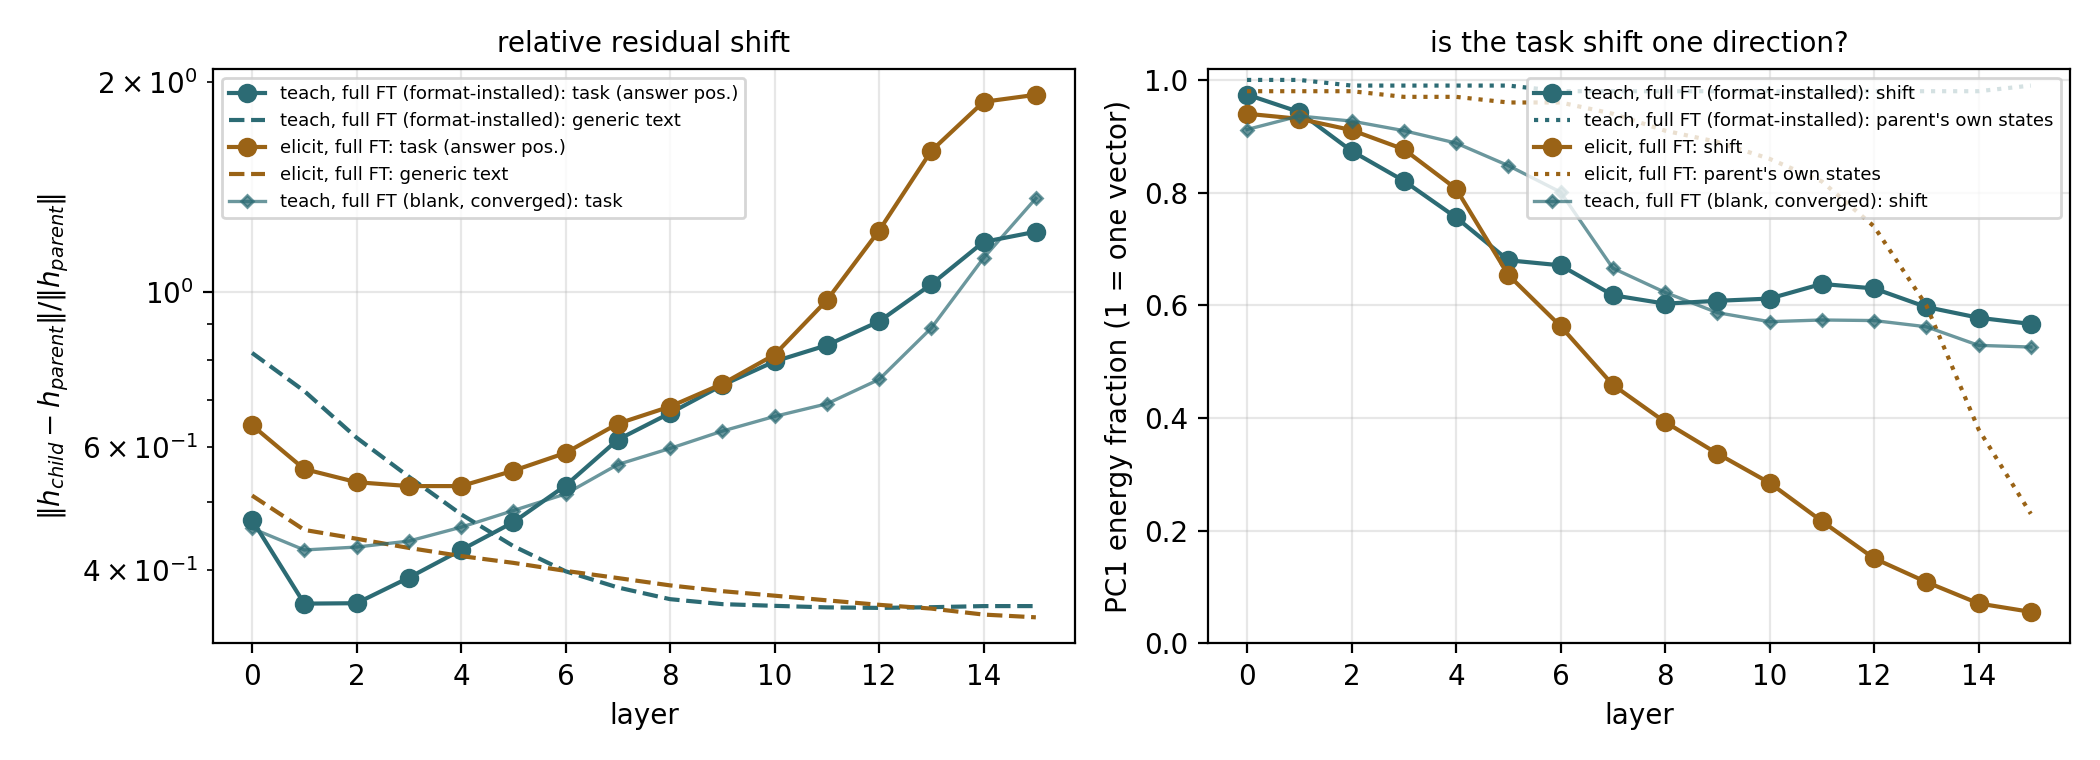
\includegraphics[width=0.95\textwidth]{figures/fig_resid_shift.png}
\caption{The pair (thick) with the blank-base taught control (thin diamonds). Left: relative residual shift by layer at the answer
position (solid) and on generic story text (dashed): the size of the change by layer. Right:
shared-direction score (PC1) of the 256 per-problem changes by layer, with the parent's own states
dotted.}
\label{fig:resid}
\end{figure}
\begin{table}[h]\centering\small
\begin{adjustbox}{max width=\textwidth}
\begin{tabular}{lccc}
\toprule
 & \textbf{elicit FT} & \textbf{teach FT} & teach FT from the blank base (control) \\
\midrule
final exact match & 0.986 & 0.424 & 0.819 \\
shared-direction score (PC1) of the change, last layer (parent's own states) & \textbf{0.056} (0.23) & \textbf{0.567} (0.99) & 0.526 (0.98) \\
same, after removing answer-token directions & 0.061 & 0.561 & 0.528 \\
cosine of each change to the mean change & 0.23 & 0.80 & 0.74 \\
size of the change relative to the parent's state, last layer & 1.92 & 1.22 & 1.36 \\
\bottomrule
\end{tabular}
\end{adjustbox}
\caption{Change of the internal state parent$\to$child at the answer position, 256 problems,
fp32. Under LoRA (1M elicit / 4M teach from the blank base): score 0.063 vs 0.528, unchanged
after removing the answer directions; the LoRA-taught size is $29\times$ (an adapter artefact).}
\label{tab:resid}
\end{table}

% =====================================================================
\end{enumerate}
\section*{D. The latent state: what it means and what it permits before training}
\begin{enumerate}[label=\textbf{M\arabic*}, leftmargin=*, itemsep=1.2em, resume]

\metricsec{Latent reach}{do the words already reach the machinery?}
\what{Before any target training, does a natural-language question already put the arithmetic
components into a problem-specific state (elicit), or is there nothing for the words to reach
(teach)?}
\how{Render each problem two ways --- \texttt{What is the sum of 621 and 5068?} and
\texttt{621 + 5068 = } --- and record every node's activation at the answer position. Per node:
the mean cosine between the two renderings of the \emph{same} problem minus the mean cosine
between renderings of \emph{different} problems (the ``bridging index''). Positive means the
words put the node into the state the symbols put it in. MLP blocks only: attention heads share
digit tokens across renderings and would score trivially. Compared between the symbol-only
engine (no binding dose) and the elicit parent (binding dose installed). A second, geometry-only
check: how problem-specific the answer-position state itself is, as PC1 and cosine-to-mean across
the 256 problems ($\approx1$ means the same state for every problem).}
\numbers{Bridging index of the arithmetic MLPs on natural-language input: $\approx0$ in the
symbol-only engine, $+0.07$--$0.13$ across layers 7--15 in the elicit parent ($10\times$). Shared-direction score of the parent's own answer-position states: $0.23$ (elicit parent,
problem-specific) vs $0.99$ (teach parent; the blank base $0.98$) --- the same state for every
problem (Table~\ref{tab:resid}, ``parent's own states''). \emph{Reading:} the words already reach the elicit parent's machinery
before any target training; the teach parents have nothing for them to reach.}

\metricsec{Answer depth}{the answer already there vs.\ absent; finished one layer earlier vs.\ later}
\what{Is the answer readable from the parent's internal state before it can say it (elicit) or
absent (teach); and after training, is it finished one layer earlier (elicit) or later (teach)?}
\how{Read the model's intermediate state at each layer as if it were the output, three ways.
\emph{Logit lens}: apply the final unembedding to the layer-$\ell$ state. \emph{J-lens}
(Jacobian lens): first transport the state to the final-layer basis with the average Jacobian
$\partial h_{\mathrm{final}}/\partial h_\ell$ over held-out story text, then unembed --- this
reads what the state is \emph{disposed to make the model say}, and is where the answer can appear
before the model emits it. \emph{R-lens}: the same transport with a relevance-propagation
backward pass, more faithful at early layers. Scored token $=$ the first digit chunk of the
answer (for negative answers the sign is fed in first, so predicting a minus sign never counts).
Per layer: the answer token's median rank among 128K vocabulary entries (chance 64K); the
\emph{logit-diff}, the model's preference for the correct answer over a mismatched problem's
answer, in nats ($0$ $=$ no answer-specific signal); and the \emph{settled depth}, the first
layer from which the token stays top-ranked to the end. Rank without logit-diff can be a number
prior (any number ranks well in a model that emits numbers); the two are read together.}
\numbers{Figure~\ref{fig:lens}, Table~\ref{tab:lens}. Before training: the elicit parent
ranks the answer $174$ of 128K in its output and $510$ at layer 14 (J-lens), preferring it by
$2.1$ nats while it emits a rewrite; the teach parent ranks it $452$ but with logit-diff $0.0$ at
every layer --- a number, not this number (the blank base: rank $\sim75$K, logit-diff $0.0$).
After training: the elicited child settles at layer 14 (J-rank $338$ / $8$ / $1$ at layers 12 /
13 / 14), the trajectory of the parent's engine on symbols ($122$ / $6$ / $1$); the taught child
settles at layer 15 ($27{,}044$ / $15{,}058$ / $961$), as does the taught child from the blank
base. \emph{Reading:} the elicit parent already carries the answer and elicitation amplifies the
read-out; the teach parent carries nothing, and a taught model finishes the answer one layer later
even when it solves the task.}
\begin{figure}[h]\centering

\includegraphics[width=0.95\textwidth]{figures/fig_lens_depth.png}
\caption{J-lens read-out of the answer token by layer: median rank (left, chance 64K) and
logit-diff against a mismatched problem's answer (right). Gold = elicit (parent: squares; child:
diamonds; dotted: the parent on the symbol surface), teal = teach (parent: up-triangles; child:
down-triangles), grey = blank base.}
\label{fig:lens}
\end{figure}
\begin{table}[h]\centering\small
\begin{adjustbox}{max width=\textwidth}
\begin{tabular}{llccccc}
\toprule
model & surface & own acc & rank L12 (logit / J / R) & rank L14 (logit / J / R) & read-out & ld \\
\midrule
\textbf{elicit parent} & NL & 0.047 & 5{,}704 / 2{,}606 / 2{,}730 & 436 / 510 / 424 & 174 & $+2.1$ \\
\textbf{teach parent} (format-installed) & NL & 0.004 & 8{,}394 / 4{,}036 / 5{,}417 & 1{,}106 / 997 / 998 & 452 & $0.0$ \\
\textbf{elicited child} (FT) & NL & 0.988 & 1{,}797 / 338 / 492 & 1 / 1 / 1 & 1 & $+18.7$ \\
\textbf{taught child} (FT) & NL & 0.535 & 23{,}909 / 27{,}044 / 25{,}529 & 381 / 961 / 1{,}848 & 1 & $+14.2$ \\
\midrule
blank base & NL & 0.000 & 76{,}049 / 80{,}840 / 78{,}243 & 77{,}707 / 77{,}320 / 79{,}116 & 75{,}441 & $0.0$ \\
taught child from the blank base (FT) & NL & 0.844 & 18{,}988 / 4{,}123 / 9{,}620 & 170 / 138 / 459 & 1 & $+16.1$ \\
elicit parent (the engine) & symbols & 0.836 & 1{,}224 / 122 / 334 & 1 / 1 / 1 & 1 & $+15.1$ \\
\bottomrule
\end{tabular}
\end{adjustbox}
\caption{Median rank of the answer's first digit token among 128K entries under the three lenses;
``own acc'' $=$ the model's own first-digit-token accuracy on the 256 problems; read-out $=$ the
last layer, where all lenses equal the model's output; ld $=$ logit-diff at the read-out (nats).
Bottom: the blank base (rank without a number prior), the taught child from it (settles at layer
15 too), and the engine's own trajectory on symbols, which the elicited child reproduces.}
\label{tab:lens}
\end{table}

\metricsec{Switch-on by patching}{can the capability be turned on without training?}
\what{With the parent's weights frozen, does writing the fine-tuned child's internal activations
into the parent make it solve the task --- possible only if the machinery is already there
(elicit) and impossible if it is not (teach)?}
\how{Donor patching. Take the fine-tuned child (the donor) and its parent (the patient). For each
problem, run the child and record its activations at the 32 circuit nodes of M2 at the answer
position; run the parent on the same problem and overwrite those 32 activations with the child's;
let the parent finish. Two variants: \emph{per-prompt states} (each problem gets the child's
activations on that problem) and \emph{mean vector} (every problem gets the child's average
activation, a single constant shift). Control: the same with 32 random nodes. Read-outs: exact
match, and ``format'' $=$ the fraction of outputs that are a number at all. Done for the elicit
side (elicited child into the elicit parent) and the teach side (each taught child into its own
parent: the blank base, or the format-installed base).}
\numbers{Table~\ref{tab:steer}, Figure~\ref{fig:ladder}. Elicit parent: the child's per-prompt
states patched into 32 nodes give exact match $0.121$ from a parent that scores $0.000$ (random
nodes $0.000$; the mean vector changes only the output format). Teach parent: its child's states
patched in give $0.016$ (into the blank base, from the blank-base child: $0.004$).
\emph{Reading:} 32 activations from the child are enough to switch the latent capability on
because the machinery underneath is the parent's own; the same patch from a taught child finds
nothing underneath in its parent.}
\begin{table}[h]\centering\small
\begin{adjustbox}{max width=\textwidth}
\begin{tabular}{llcc}
\toprule
Patient + donor (32 circuit nodes) & condition & format & exact match \\
\midrule
\textbf{elicit parent + elicited child's per-prompt states} & circuit nodes & 0.387 & \textbf{0.121} \\
\textbf{teach parent + taught child's per-prompt states} & circuit nodes & 0.836 (parent 1.000) & \textbf{0.016} \\
\midrule
elicit parent + LoRA child's per-prompt states & circuit nodes & 0.359 & 0.125 \\
 & random-32 nodes & 0.051 & 0.000 \\
elicit parent + LoRA child's mean vector & circuit nodes & 0.164 & 0.000 \\
blank base + blank-base taught child's states & every condition & $\le$0.02 & $\le$0.004 \\
\bottomrule
\end{tabular}
\end{adjustbox}
\caption{Donor patching, weights frozen. The parents score 0.000 unpatched. Bottom: controls
(random nodes, the mean vector, the LoRA child as donor, the blank-base pair).}
\label{tab:steer}
\end{table}
\begin{figure}[h]\centering
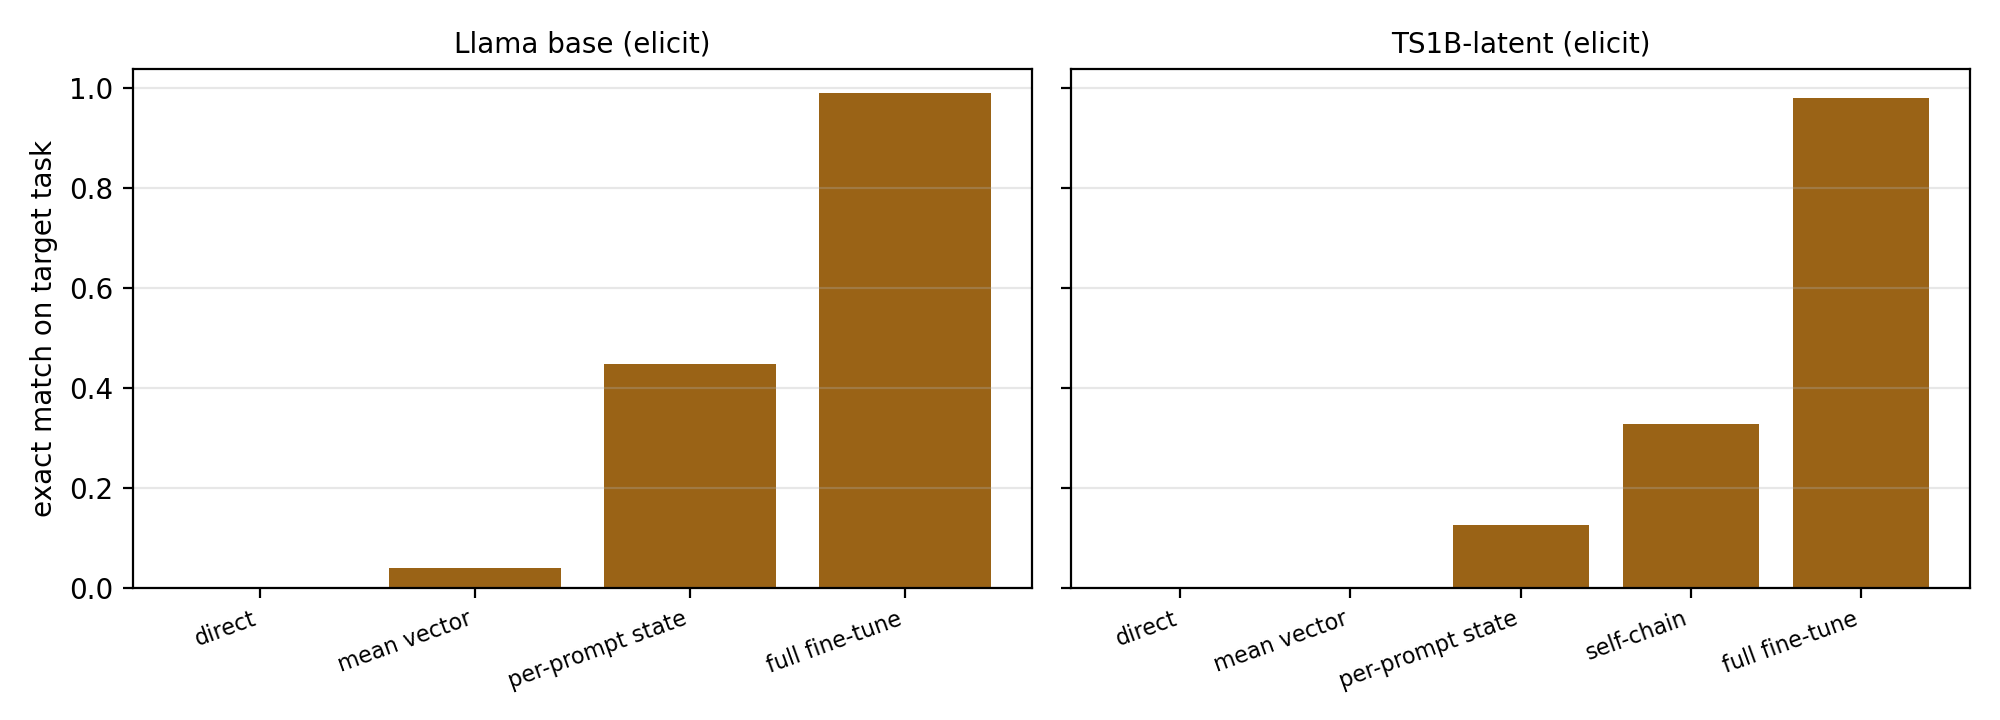
\includegraphics[width=0.75\textwidth]{figures/fig_intervention_ladder.png}
\caption{Donor patching on the elicit parent (right; left: the same on a Llama-3.2-1B parent,
for intuition), weights frozen except the last bar: direct, mean vector, per-prompt states, and
the fine-tuned child for scale; the self-chain bar is the construction check of
Table~\ref{tab:premise}, not a patch.}
\label{fig:ladder}
\end{figure}

\end{enumerate}

% =====================================================================
\section*{E. Every metric on one page}

The pair, one row per metric; the third column is the taught twin fine-tuned from the blank base
with the same recipe, the robustness check: it performs better ($0.819$) and agrees with the
format-installed taught twin on every row.

\begin{table}[h]\centering\small
\begin{adjustbox}{max width=\textwidth}
\begin{tabular}{lcccl}
\toprule
 & \textbf{elicit FT} & \textbf{teach FT} & teach FT from the blank base & metric \\
\midrule
exact match (0-shot) & 0.986 & 0.424 & 0.819 & M1 \\
steps to stop (passes) & 21{,}500 (0.7) & 58{,}500 (1.9) & 72{,}000 (2.3) & M1 \\
held-out test loss (nats/token) & 0.015 & 0.639 & 0.154 & M1 \\
circuit overlap with the parent's own circuit & 0.391 (parent ceiling 0.306) & undefined (parent map is noise) & undefined & M2 \\
circuit overlap with the elicited circuit & -- & 0.306 & 0.333 & M2 \\
operand-reading heads vs the engine's (first / second) & 0.694 / 0.857 & 0.879 / 0.659 & 0.763 / 0.658 & M3 \\
gradient norm, first 1\% $\to$ last 10\% of steps & 4.80 $\to$ 1.39 (decays 3.4$\times$) & 2.69 $\to$ 3.77 (grows 1.4$\times$) & 2.30 $\to$ 3.43 (grows 1.5$\times$) & M5 \\
cumulative gradient mass & 44{,}021 & 378{,}170 & 353{,}277 (+ 30{,}954) & M5 \\
relative weight write $\|\Delta W\|/\|W\|$ & 0.050 & 0.086 & 0.102 & M6 \\
shared-direction score of the state change (after removing answer content) & 0.056 (0.061) & 0.567 (0.561) & 0.526 (0.528) & M7 \\
answer settled depth, median (quartiles) & layer 14 (14--14) & layer 15 (15--15) & layer 15 (15--15) & M9 \\
J-space rank of the answer at layers 12 / 13 / 14 & 338 / 8 / 1 & 27{,}044 / 15{,}058 / 961 & 4{,}123 / 1{,}832 / 138 & M9 \\
child's states patched into its own parent, per-prompt (mean) & 0.121 (format only) & 0.016 (0.000) & 0.004 (0.000) & M10 \\
\bottomrule
\end{tabular}
\end{adjustbox}
\caption{The pair and the blank-base robustness check, one row per metric.}
\label{tab:ftpair}
\end{table}

\section*{Notes on measurement}

\begin{itemize}[nosep]
  \item \textbf{Every circuit is load-bearing (a check, not a metric: it does not separate the
    regimes).} True activation patching --- copy the top-$k$ nodes' clean activations into a
    corrupted run (sufficiency) or corrupt them in a clean run (necessity), 128 problem pairs ---
    gives top-8 of 528 nodes recovering / destroying the answer at $0.923$ / $0.943$ (elicit FT)
    and $0.983$ / $0.988$ (teach FT), top-32 $\ge0.996$ for both. The overlaps in M2 compare two
    real mechanisms.
  \item \textbf{Teach-side metrics are measured on a taught model that solves the task.} The
    first taught endpoint (LoRA 1M, exact match 0.093) had not learned it. Every teach-side
    metric was re-run on fully fine-tuned taught endpoints (from the format-installed and the
    blank base), with the fully fine-tuned elicited endpoint as the method control. Three earlier
    readings changed and are stated in their revised form above: taught operand roles are mostly
    shared rather than absent (M3), the circuit difference is partial rather than total (M2), and
    the size of the taught state change follows the fine-tuning method (M7).
  \item \textbf{Answer depth is scored on the first digit token.} Scoring the raw first token
    credited a taught child with layer-5 formation on 48 problems --- all subtractions with a
    negative answer, whose first token is the minus sign, produced by a comparison circuit. With
    the sign fed in first the effect vanishes; the other models were unaffected.
  \item \textbf{Construction controls.} The same doses on the blank twin change nothing on the
    target (0.000 in every probe); a sum-only binding dose leaves ``difference'' unbound; the
    composition law self-chain $=$ rewrite $\times$ compute held on four variants.
\end{itemize}

\end{document}
